%!TEX root = ../dissertation.tex

%\begin{savequote}[75mm]
%
%\qauthor{someone}
%\end{savequote}


\chapter{Chapter 6 Calculations}
\label{appendix:Ch6Cal}

\section{$\Delta x$ : Time Scaling Behavior (Power Law 12-Sites)}

In order to quantify the transport distance of the particles, we defined the first moment of the two-point-density-correlation distribution, $\Delta x = 2 \sum_d G_2(d) \times  d$ where $G_2(d) = \langle n_i n_{i+d} \rangle_{i,\phi} - \langle n_i \rangle_{i,\phi} \langle n_{i+d} \rangle_{i,\phi}$, $i$ is the site index, and $\phi$ is the disorder realization. Numerical simulations were performed to determine time-scaling behavior of the first moment (Fig.~\ref{fig:logFit}).

\begin{figure}[t!]
	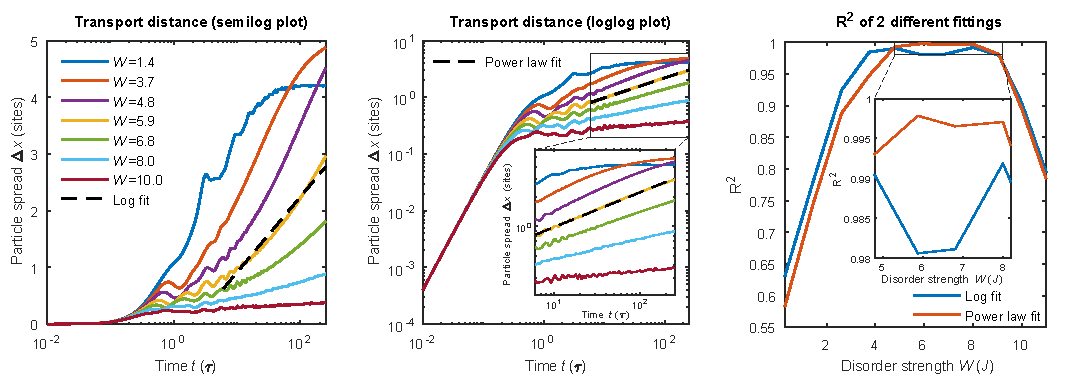
\includegraphics[width=\columnwidth]{figures/ch6/logFit.pdf}
	\caption{\textbf{Two different fittings for the time-dependence of the transport distance at various disorder strengths.} The left panel and the center panels show the time dependence of the particle spread $\Delta x$ in a 12-site system for various disorder strengths in semi-log and log-log scales. The dashed lines are sample least-square fits assuming logarithm and power-law time scaling, respectively. The right panel shows the R$^2$ values of each fit as a function of disorder strength. All simulations were performed by exact numerical integration of Schr\"{o}dinger's equation, as described in the previous section.
	}
	\label{fig:logFit}
\end{figure}

To characterize the correct functional form of the temporal transport behavior of the system, we fit the first moment to either a logarithmically slow growth in time or a power-law growth in time. We look at times that avoid the initial transient dynamics in the system $t/\tau> L/2$ (the time for relaxation in the non-disordered, $W=0$, case). Since we only experimentally measure up to a final evolution time of $t=100\tau$, we restrict our fitting of the temporal transport behavior in the system to $L/2<t/\tau\leq100$. This time range was found to be robust to change in the exact endpoints. Additionally, we can see in Fig.~\ref{fig:logFit} that only disorder strengths $W\gtrapprox4.8J$ appear unaffected by the system's finite size at $t=100\tau$. We therefore expect that comparing the fit quality in the critical disorder regime ($5\lessapprox W/J \lessapprox 8$) is a good metric for determining which functional form of the temporal transport behavior. We find, by looking at the $R^2$ metric of the fits in this region, that the transport behavior more closely relates to a power-law rather than a logarithmically slow growth. Hence, in this paper, we assumed a power-law time scaling of the particle spread to analyze the data.

\section{Spectral Statistics}

\begin{figure}
\floatbox[{\capbeside\thisfloatsetup{capbesideposition={left,top},capbesidewidth=2 in}}]{figure}[\FBwidth]
{\caption{\textbf{Spectral Statistics.} This shows the spectral statistics ratio, $\langle r \rangle \equiv \langle \frac{\mathrm{min}(\Delta_n,\Delta_{n+1})}{\mathrm{max}(\Delta_n,\Delta_{n+1})} \rangle$, for system sizes of L=6 and L=8. The approximate crossing point is $W\approx5J$ which bounds the critical point from below $W_c\gtrapprox5J$ and is consistent with the experimentally observed point of departure from thermalization.} \label{fig:RStat}}
{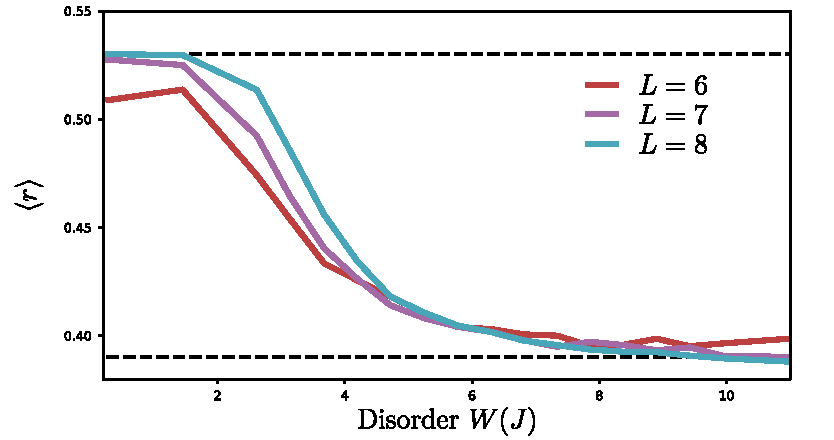
\includegraphics[width=4 in]{figures/ch6/figS6/RStat.pdf}} 
\end{figure}

The spectral statistics ratio ($r$) is a common metric used to determine the transition from the thermalizing to many-body-localized behavior. This ratio is defined as $r\equiv \mathrm{min} \{ \Delta_n , \Delta_{n+1} \} / \mathrm{max} \{ \Delta_n, \Delta_{n+1} \}$, where $\Delta_n = E_n - E_{n+1}$ is the spacing between eigenenergies in the system. This is then averaged over the eigenstates that do not lie close to the ends of the spectrum. In this case, we average over the middle 2/3 of the eigenstates. This ratio is sensitive to the test of level repulsion of the system, which a hallmark of a thermalizing system. This ratio approaches the Gaussian orthogonal ensemble (GOE) value of $r\approx 0.53$ in the thermalizing regime and approaches the Poisson value of $r\approx 0.39$ in the localized phase. We are able to compute these via exact diagonalization for system sizes up to L=8. The crossing point for successively larger system sizes is a typical method for helping estimate the lower bound for the critical point for the transition. With our experimental realization of the quasi-periodic potential, we see a cross point at $W\approx5J$ which bounds the critical point in the thermodynamic limit from below $W_c\gtrapprox 5J$ \cite{Khemani2017}.

%\begin{figure}[h!]
%	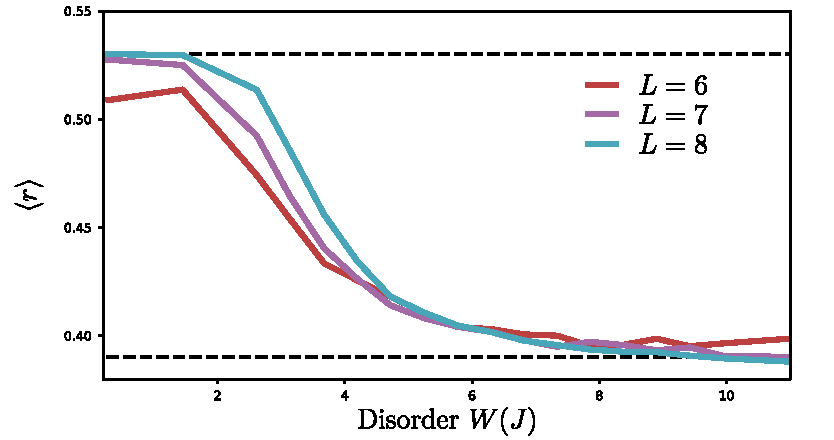
\includegraphics[width=4 in]{figures/ch6/figS6/RStat.pdf}
%	\caption{\textbf{Spectral Statistics.} This shows the spectral statistics ratio, $\langle r \rangle \equiv \langle \frac{\mathrm{min}(\Delta_n,\Delta_{n+1})}{\mathrm{max}(\Delta_n,\Delta_{n+1})} \rangle$, for system sizes of L=6 and L=8. The approximate crossing point is $W\approx5J$ which bounds the critical point from below $W_c\gtrapprox5J$ and is consistent with the experimentally observed point of departure from thermalization.}
%	\label{fig:RStat}
%\end{figure}


\section{Enhanced Thermalization}

\begin{figure}
\floatbox[{\capbeside\thisfloatsetup{capbesideposition={left,top},capbesidewidth=2 in}}]{figure}[\FBwidth]
	{\caption{\textbf{Numeric Integration of Fluctuations 12 vs 8.} This plot shows the integrated fluctuations of the exact numeric theory (solid lines) and measured data (points) for the curves from Fig.~2c. Only a subset of points were used that were measured at the same disorder value in both the twelve-site and eight-site experiments. The numerical integration was evaluated via the trapezoid rule. The relevant metric is the final point that incorporates the integral of all points along the curve and provides a robust metric for showing enhanced thermalization in the larger system. This integrated difference exceeds the null-hypothesis by more than two standard error bars of the mean.
	}
	\label{fig:TrapzInt}}
{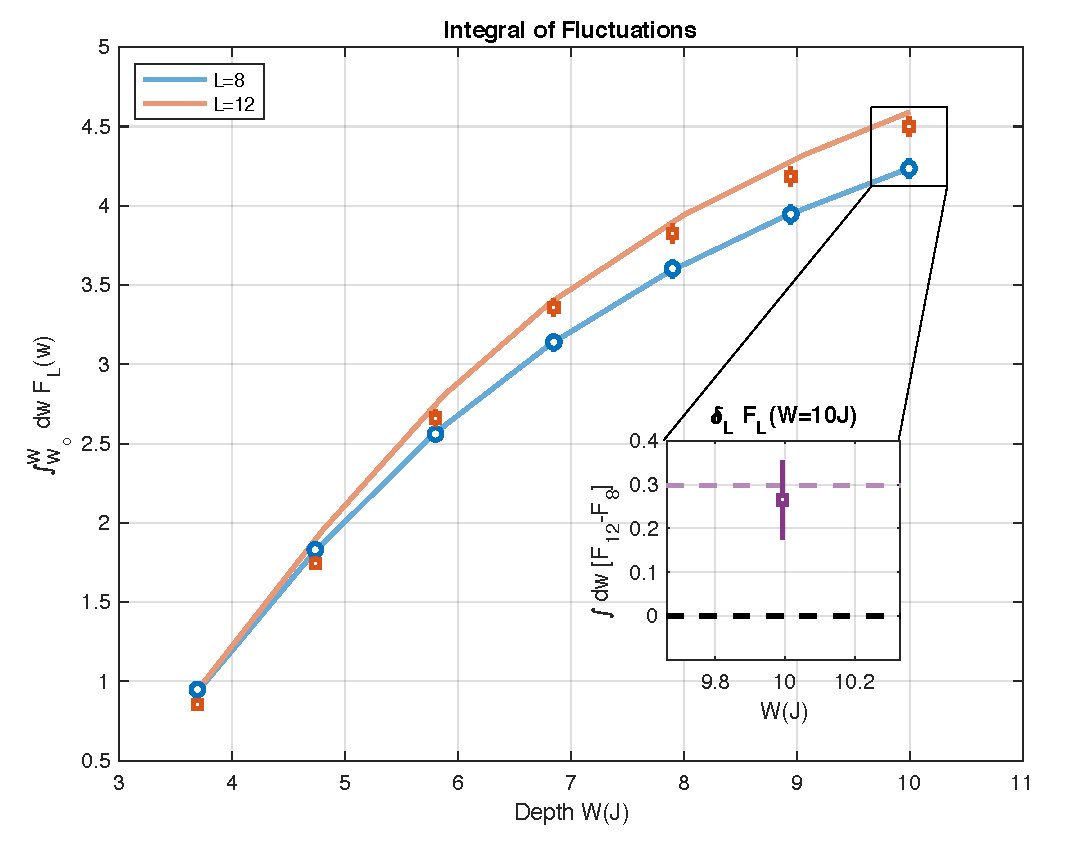
\includegraphics[width=4 in]{figures/ch6/figS5/IntegralPlotv2.pdf}} 
\end{figure}

The measured on-site number fluctuations plotted in \S \ref{sec:ch6} (Fig.~\ref{fig:crTherm}) show enhanced thermalization in the larger system across an intermediate disorder range which we use to identify the critical regime. To provide a more robust metric of the enhanced thermalization in the larger system-size, we numerically integrate the two curves and compare the difference in the fluctuations. This final integrated difference is plotted in Fig.~\ref{fig:TrapzInt}. The inset quantifies the systematically enhanced thermalization in the larger system size where it exceeds the null hypothesis by more than two standard errors of the mean.

%\begin{figure}[h!]
%	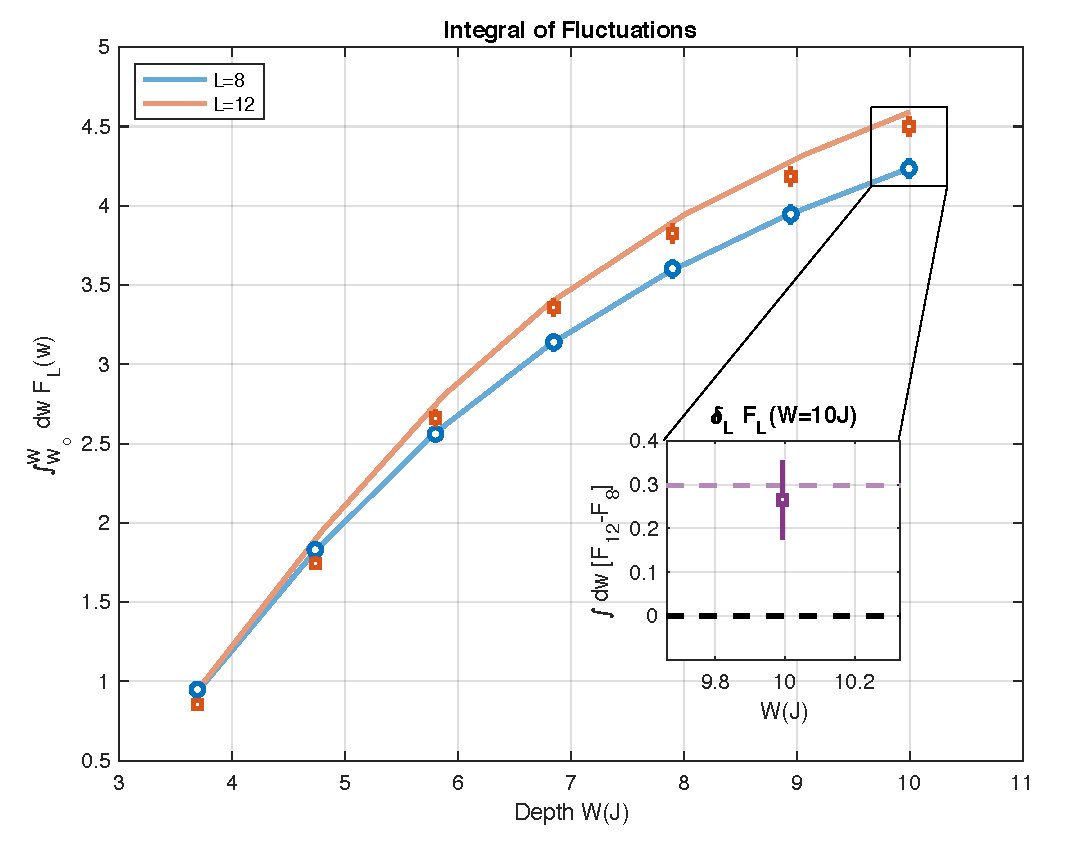
\includegraphics[width=4 in]{figures/ch6/figS5/IntegralPlotv2.pdf}
%	\caption{\textbf{Numeric Integration of Fluctuations 12 vs 8} This plot shows the integrated fluctuations of the exact numeric theory (solid lines) and measured data (points) for the curves from Fig.~2c. Only a subset of points were used that were measured at the same disorder value in both the twelve-site and eight-site experiments. The numerical integration was evaluated via the trapezoid rule. The relevant metric is the final point that incorporates the integral of all points along the curve and provides a robust metric for showing enhanced thermalization in the larger system. This integrated difference exceeds the null-hypothesis by more than two standard error bars of the mean.
%	}
%	\label{fig:TrapzInt}
%\end{figure}


\section{Subsystem-size fluctuations scaling}

As discussed in \S \ref{sec:ch6}, the subsystem-size scaling of particle-number fluctuations is a proposed probe for investigating the thermal-to-MBL transition. In the infinite temperature case (all Fock basis states contributing equally), the probability of fluctuations can be found easily by considering the number of states possible in a subsystem of size $L_A$ with $n_A$ particles:

\[
\mathcal{D}_A = \left ( \frac{(n_A + L_A - 1)!}{ n_A! (L_A -1)! } \right )
\] 

where its complement is given by $\{ L_B = L-L_A$, $n_B = N-n_A \}$ where $L$ is the total system size and $N$ is the total atom number. This gives rise to the probability of having $n_A$ atoms in subsystem size of $L_A$:

\[
P(n_A,L_A, N)_L = \left (\frac{(n_A + L_A - 1)!}{ n_A! (L_A -1)! } \right ) \left (\frac{(N-n_A + L- L_A - 1)!}{ (N-n_A)! (L-L_A -1)! } \right ) \Big / \left (\frac{(N+L- 1)!}{ N! (L -1)! } \right ) 
\]

The fluctuations for such a distribution is then calculated as the second moment of $n_A$:

\begin{equation}
F(L_A, N)_L = \sqrt{\left ( \sum_{n_A=0}^N P(n_A) n_A^2 \right ) - \left ( \sum_{n_A=0}^N P(n_A) n_A^2 \right )^2}
\end{equation}

This reduces to the familiar form of the Bernoulli distribution with an additional enhancement factor that derives from indistinguishable bosonic statistics:

\begin{equation}
\label{eqn:FNL}
F(L_A,N)_L/N = \left ( \frac{\left ( L-L_A \right ) L_A }{L^2} \right ) \left ( \frac{ 1+N/L }{ 1+1/L } \right )
\end{equation}

In the limit where we have integer filling, $N=\nu L$, we can see the scaling more easily for the fluctuations per particle $\tilde{\mathcal{F}}(l,\nu)_L$:

\begin{equation}
\label{eqn:FNL2}
\tilde{\mathcal{F}}(L_A,\nu)_L = \left ( \frac{\left ( L-L_A \right ) l }{L^2} \right ) \left ( \frac{ 1+\nu }{ 1+1/L } \right )
\end{equation}

In the large $\{N,L_A,L\}$ limits, the probability of particle number becomes approximately Gaussian with a mean $\mu_{n_A} = N \times L_A/L$ and varince $\sigma_{n_A}^2 = N^2 \frac{(L_A)(L-L_A)}{L^2}$

This Gaussian relationship allows for a simple relationship to the number entropy that is approximately logarithmic in a given system size by evaluating the von Neumann entropy of particle number:

\begin{equation}
S_n (L_A) = - \sum_{n_A=0}^N P(n_A,L_A, N)_L \log [P(n_A,L_A, N)]
\end{equation}

The derivation of the Bernoulli distribution relies on particles being uniformly distributed throughout the system. This also means that the probability of a particle living in $L_A$ is just given by:

\[
P(L_A)=\int_{l=0}^{L_A} \frac{1}{L} d{l}
\] 

In the case that disorder is now applied to the lattice, this would have to be modified fundamentally since the particles then live in exponentially localized orbitals with a characteristic localization length $\xi$.  We find phenomenologically that this modifies the probability of $P(n_A)$ from a Gaussian, but an exponential:

\[
P(n_A,L_A,N)_L \sim e^{-(n_A-N \frac{L_A}{L})/\xi}
\]

Due to this similarity, we attempted an approximation of fluctuations in the localized regime by $\sim \cosh[L_A/\xi]$. In the two extremes, $(\xi\rightarrow \infty, \xi\rightarrow 0)$, this form provides the correct shapes of a parabola and a constant scaling for the particle-number fluctuations, respectively. This is shown qualitatively in Fig.~\ref{fig:fScaling} as a function of time.

\begin{figure}[ht!]
		\includegraphics[width=\columnwidth]{figures/ch6/fig2v4_a.pdf} 
		\caption{\textbf{Fluctuations Scaling Behavior. a)}  The probability of particle number $n_A$ is plotted for both a subsystem size of two sites (teal) and four sites (purple). The relationship to the growth in the width of the particle number probability as a function of time is shown in the histograms as well as schematically by the shaded green triangle. \textbf{b)} The particle number fluctuations as a function of subsystem size and time in the color plot. Cross section of the fluctuations are plotted for three different evolution times: $t=1\tau$ (blue), $t=10\tau$ (purple), and$t=100\tau$ (red). }
		\label{fig:fScaling}	
\end{figure}

